\documentclass{article}

\usepackage{ctex}
\usepackage{amsmath}
\usepackage{amssymb}
\usepackage{ulem}
\usepackage{graphicx}
\usepackage{fancyhdr}
\usepackage[left=2.5cm,right=2.5cm,top=3cm,bottom=3cm]{geometry}

\pagestyle{fancy}
\fancyhf{}
\cfoot{\thepage}

\renewcommand\footrulewidth{0.6pt}
\renewcommand\figurename{图}
\renewcommand\tablename{表}
\renewcommand\contentsname{目录}
\renewcommand\refname{参考文献}

\title{安卓 Socket API 调研\footnote{编程环境为Android Studio} }
\author{王轩}

\begin{document}

\maketitle
\tableofcontents

\section{申请网络权限}
为了使用Socket API,首先需要申请网络使用权限,
在项目的AndroidManifest.xml的manifest标签下添加以下标签:
\begin{verbatim}
<uses-permission android:name="android.permission.INTERNET"/>
\end{verbatim}

\section{Socket最简单的例子}

以下是一个Socket的最简单的例子,
函数SocketHttpTest() 向202.38.64.40(test.ustc.edu.cn) 发送一个HTTP请求,
获得响应后将原始响应报文作为字符串返回。
虽然简单,但是包含了socket创建、使用、关闭等关键步骤。

\begin{verbatim}
    private String SocketHttpGetTest() {
        String msg = "";
        try{
            // 创建Socket对象,指定通信对方的IP和端口
            Socket socket = new Socket("202.38.64.40",80);
            // 获取该Socket的输入输出流
            DataOutputStream writer = new DataOutputStream(socket.getOutputStream());
            DataInputStream reader = new DataInputStream( socket.getInputStream());
            // 发送请求报文(HTTP请求头)
            writer.writeUTF("GET / HTTP/1.1\n" +
                    "Host: test.ustc.edu.cn\n" +
                    "Upgrade-Insecure-Requests: 1\n" +
                    "User-Agent: Mozilla/5.0 (Windows NT 10.0; WOW64) AppleWebKit/537.36 "+
                    "(KHTML, like Gecko) Chrome/56.0.2924.87 Safari/537.36\n" +
                    "Accept: text/html\n" +
                    "Accept-Encoding: deflate, sdch\n" +
                    "Accept-Language: zh-CN,zh;q=0.8\n\n");
            // 接受32行响应数据
            while((line=reader.readLine())!=null){
                msg += line + "\n";
            }
            socket.close();
        }catch (Exception ex) {
            return "Network Error: " + ex.toString();
        }
        return msg;
    }
\end{verbatim}

其中,最主要的步骤就是创建socket(同时指定通信对方的IP和端口),打开输入输出流,
通过对流的读写实现socket发送和接收数据。最后关闭socket。

\newpage

\section{将socket测试添加到项目}

\begin{figure}[ht]
\centering
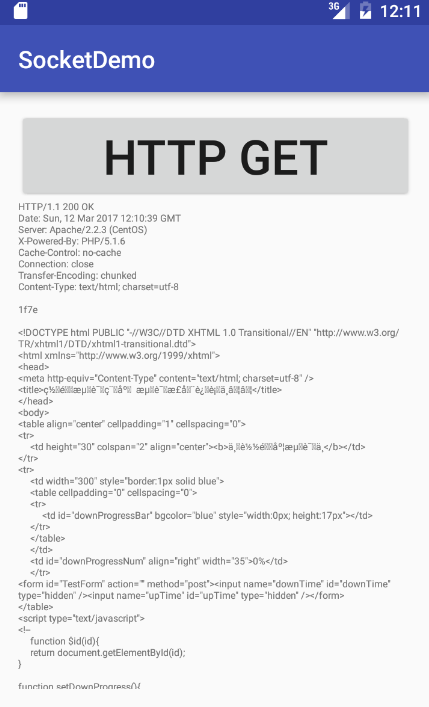
\includegraphics[width=.46\textwidth]{App.png}
\caption{测试样例App的界面}
\end{figure}

在样例App中,点击HTTP GET按钮,一段时间后会出现原始的socket响应报文。

安卓3.0以上不再允许网络操作运行在主线程(GUI线程)上,
否则运行时会抛出NetworkOnMainThreadException。
这种机制的原因是主线程负责运行GUI事件与相应,若被网络IO阻塞太久,GUI会卡顿,影响用户体验。
因此,SocketHttpGetTest()方法是需要在一个子线程调用的。

另外,socket 响应结束后被关闭,相应的线程也终止。
在终止前,为了将获得的响应字符串显示在GUI控件上,需要向主线程发送一个消息,
这需要用到Message和Handler类。

因为这不是socket API本身,此处不做赘述,详见代码。

\end{document} 
